\section{State-of-the-art BTBs and Their Limitations}
\label{hpca:sec:btbOrgs}

Prior work has proposed several BTB organizations that aim to reduce the storage cost by compressing branch targets. This section presents the most representative BTB organizations and analyzes their limitations.

\subsection{Reduced BTB} Seznec~\cite{DUPN} made a critical observation that all branch targets within a page share the same page number and only differ in page offsets. Thus, storing full target addresses in a BTB results in massive duplication of page numbers and wastage of storage capacity. To eliminate this duplication, Seznec proposed Reduced BTB (R-BTB), a variant of which was also used in ITTAGE~\cite{ittage}. The key innovation of R-BTB is to store a pointer to the page number rather than storing the page number itself in BTB. 

\Cref{hpca:fig:rbtb} presents the logical organization of R-BTB and the composition of its entries. R-BTB is composed of two partitions: Main-BTB and Page-BTB. For each branch target, apart from page offset, Main-BTB stores a pointer to the page number. The page number itself is stored in Page-BTB. If two or more branches have their targets in the same page, their Main-BTB entries will hold pointer to the same Page-BTB entry. As the number of pages is significantly smaller than number of branch targets, fewer bits are needed to hold Page-BTB pointers than page numbers themselves. Consequently, by storing a page number only once in Page-BTB, R-BTB avoids duplication and reduces storage requirements. 

\subsection{PDede}
\label{hpca:sec:pdedearch}
PDede~\cite{pdede} is the state-of-the-art BTB organization that comes with three different variants. \Cref{hpca:fig:pdede} depicts the most storage effective and best performing PDede variant, called PDede-Multi Entry Size. It improves over R-BTB in two aspects. First, it reduces the cost of storing page numbers in the Page-BTB. PDede observes that server applications, due to their large instruction footprints, touch a large number of pages thus increasing Page-BTB storage requirements. They further observe that, as different libraries get dynamically mapped to different locations in address space,  the pages tend to form spatial \emph{regions}, where a region consists of multiple contiguous pages. Just like branch targets inside a page share the same page number, the page numbers inside a region share the same region number. To eliminate the duplication of region numbers, as shown in \Cref{hpca:fig:pdede} PDede introduces a Region-BTB which stores the region number while Main-BTB stores a pointer to it just like it stores a pointer to page BTB. 

\begin{figure}
\centering
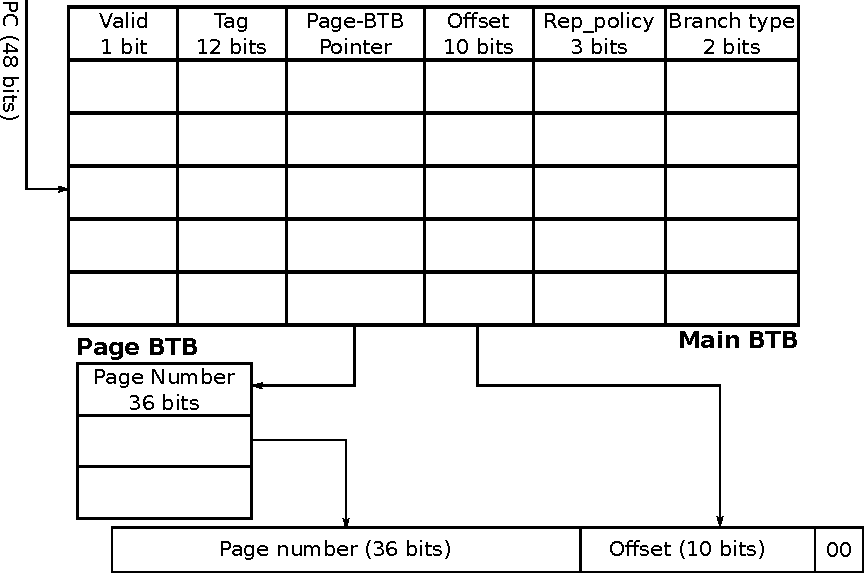
\includegraphics[width=.9\columnwidth, trim=0 0 0 0, clip]{figures/fig_9a_no_pcshift.pdf}
%\vspace{-0.1in}
\caption{Reduced BTB Organization.}
\label{hpca:fig:rbtb}
\end{figure}

Second, for the same-page branches, i.e., when the branch and its target are in the same page, PDede does not store page/region numbers as they can be recovered from branch PC. PDede reserves half of the ways in a set associate BTB for same-page branches. As the ways reserved for same-page branches do not need to store Page-BTB and Region-BTB pointers, as shown in \Cref{hpca:fig:pdedeEntry}, PDede achieves additional storage savings.

\subsection{Limitations of the state-of-the-art} Though R-BTB and PDede achieve significant storage saving by avoiding page and region number duplication, they increase BTB complexity by introducing a level of indirection and associative searches in Page- and Region-BTB. These complexities lead to increased access latency and power requirements. In addition, the state-of-the-art BTB designs are suboptimal in utilizing the available storage budget.

%\vspace{0.05in}

\subsubsection{Indirection} As Figures~\ref{hpca:fig:rbtb} and~\ref{hpca:fig:pdede} show, the access to Main-BTB only provides a part of the target address, i.e., page offset. The other parts have to be retrieved from Page-BTB and Region-BTB. Also, Page- and Region-BTB cannot be accessed in parallel with Main-BTB because the Main-BTB access provide the pointers to them. As a result, the sequential Main-BTB and Page-/Region-BTB accesses increase the overall BTB access latency. This additional latency either enforces a two-cycle BTB lookup or necessitates a longer clock period. Both of these alternatives are detrimental to performance.  PDede does avoid this indirection penalty to some extent because the same-page branches do not need to access Page-/Region-BTB rather they get their page and region number from the branch PC itself. However, the different-page branches, i.e., where branch PC and target address lie in different pages, do need to pay the indirection penalty.

\begin{figure}
\centering
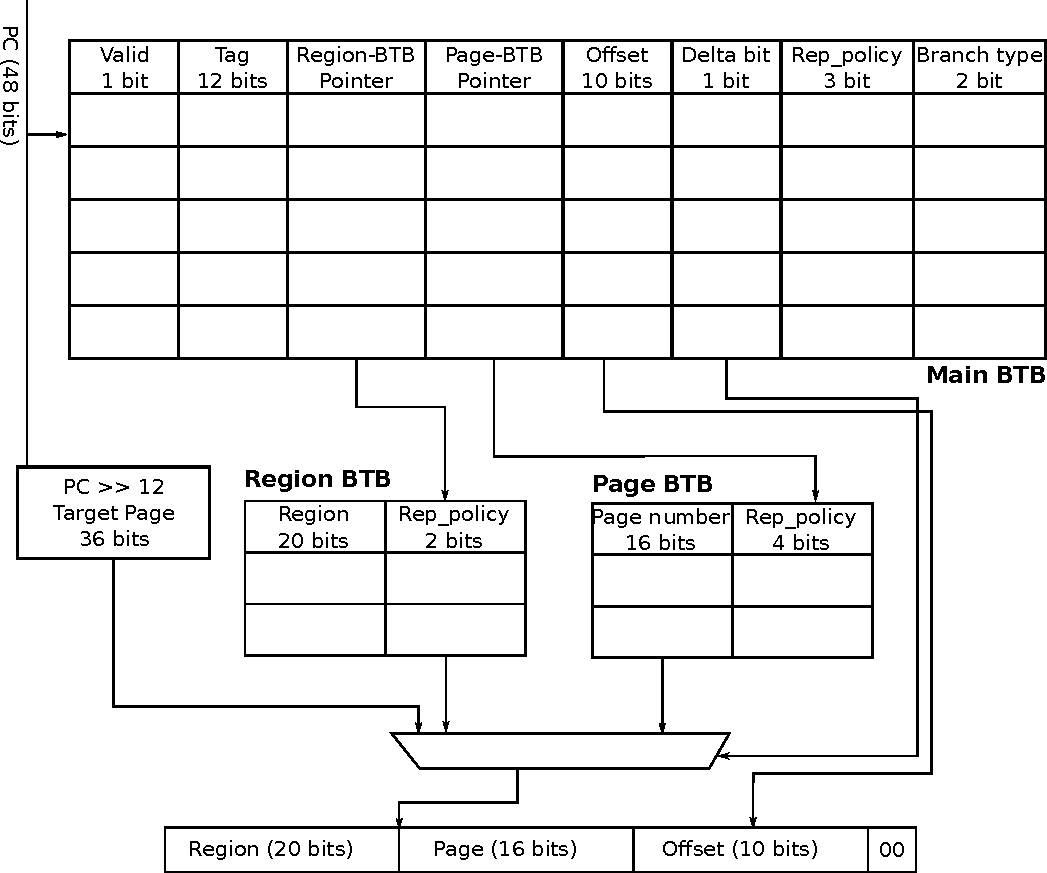
\includegraphics[width=.9\columnwidth, trim=0 0 0 10, clip]{figures/fig_9a.pdf}
\caption{PDede BTB Organization.}
\label{hpca:fig:pdede}
\end{figure}

\begin{figure}
\centering
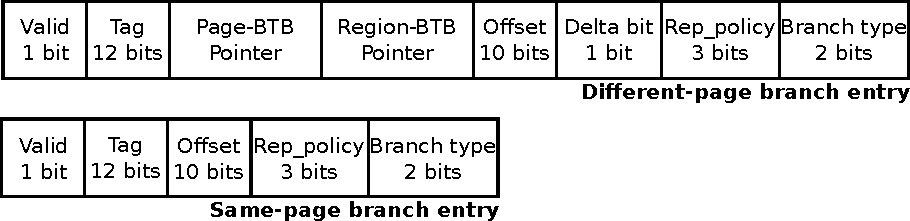
\includegraphics[width=.9\columnwidth, trim=0 0 0 0, clip]{figures/PDede_branch_entries.pdf}
\caption{Different- and same-page PDede entry composition.}
\label{hpca:fig:pdedeEntry}
\end{figure}


\begin{sidewaysfigure}
    \centering
    %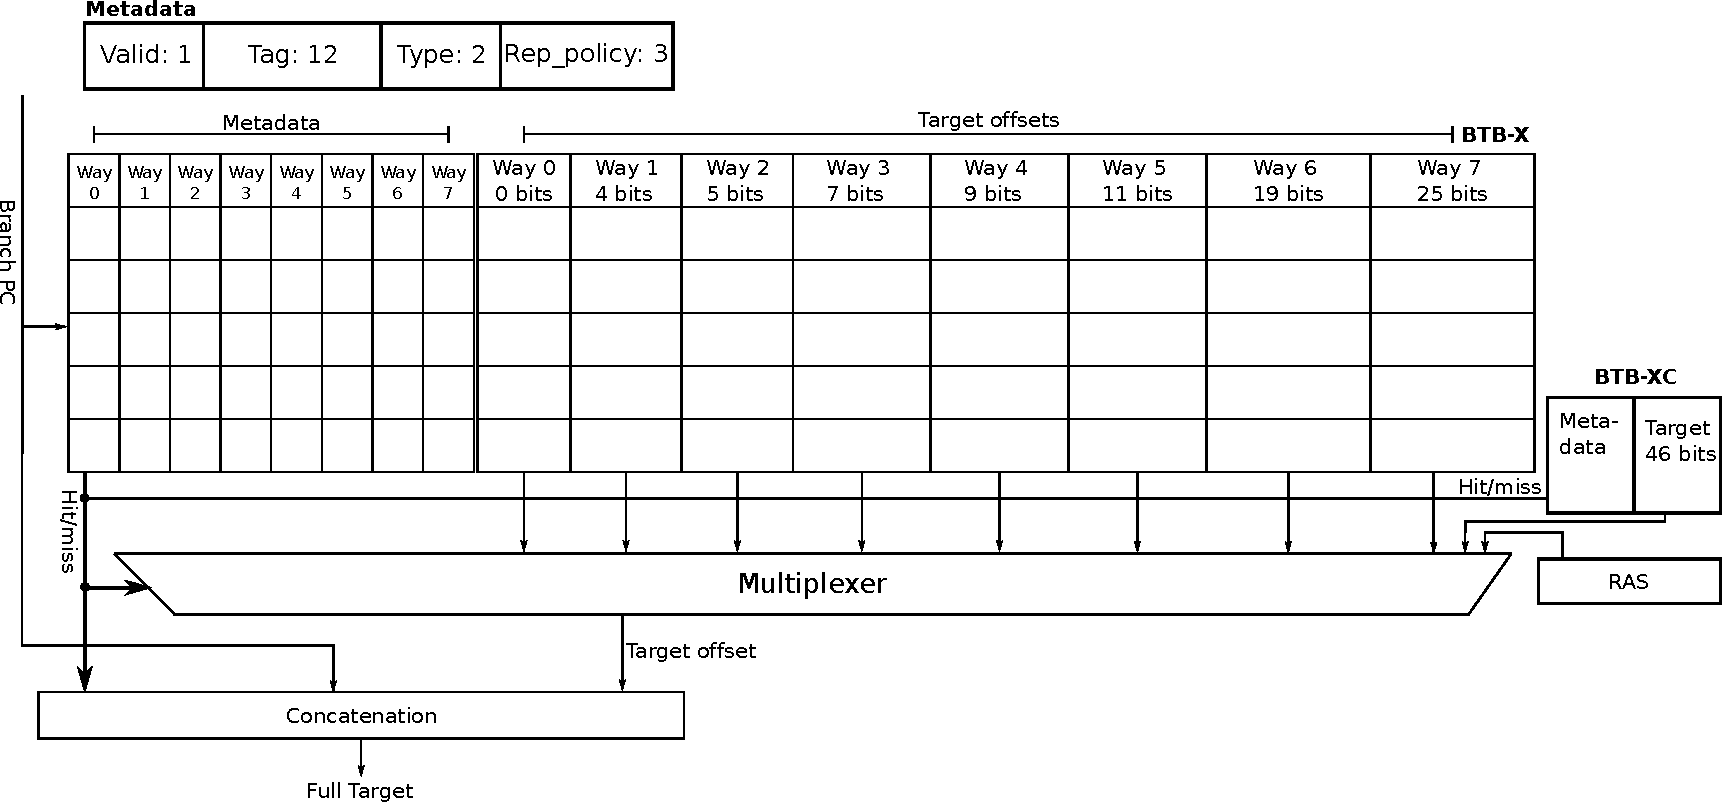
\includegraphics[width=0.7\columnwidth, trim=230 150 340 150, clip]{figures/BTB-X.pdf}
    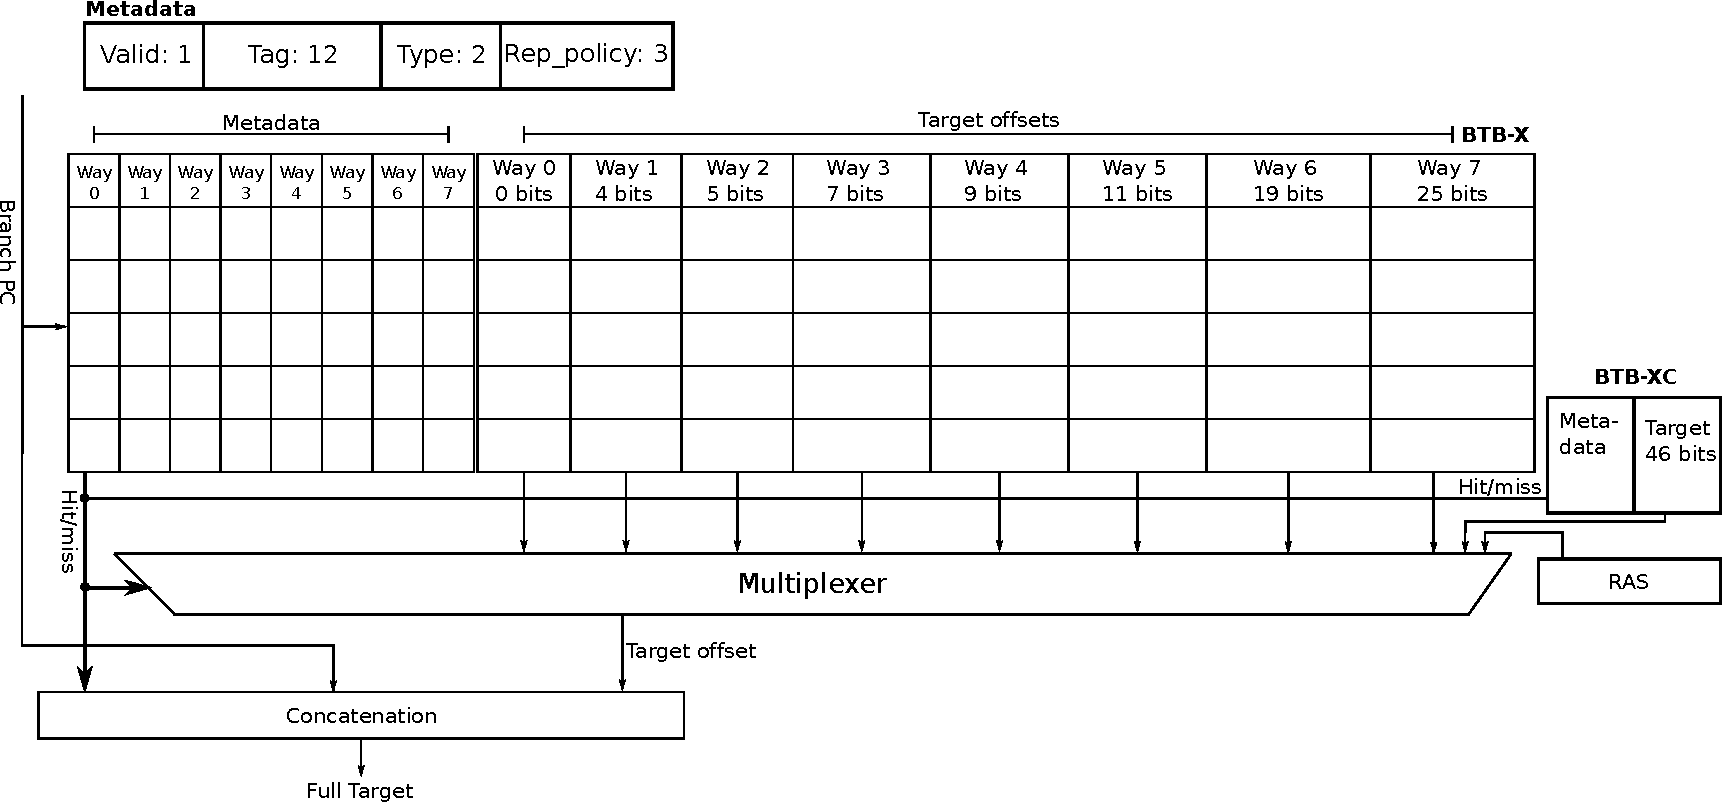
\includegraphics[width=\textwidth]{figures/BTB-X.pdf}
    \caption{BTB-X organization and entry/set composition.}
    %\vspace{-0.15in}
    \label{hpca:fig:btbx}
\end{sidewaysfigure}

%\vspace{0.05in}

\subsubsection{Associative searches} On allocating a new BTB entry, all BTB partitions (Main-BTB, Page-BTB, and Region-BTB) may need to be updated. The replacement policy chooses the entry to be replaced in Main-BTB. However, Page- and Region-BTB need to be searched to check if the page/region number for the incoming target is already present or not. As the page/region number can be present anywhere in the Page/Region-BTB, ITTAGE~\cite{ittage} uses fully-associative searches which increase the power requirements especially when the number of entries grows. PDede (partially) solves this limitation by restricting the number of entries where a page number can reside for a given branch target to 16. However, limiting the number of entries increases the likelihood of conflict misses.

\subsubsection{Suboptimal storage utilization} Though R-BTB and PDede significantly improve storage utilization over conventional BTB, they still miss plenty of opportunity. This is because, in case of R-BTB, it uses a fixed size target representation for all branches, i.e., a 10-bit offset plus a fixed sized page-BTB pointer. In contrast, our analysis of \Cref{hpca:sec:analysis} shows a large variance in target offset sizes that naturally makes the single sized organization of R-BTB storage inefficient as it needs to be sized for the largest target offset. For example, as shown by \Cref{hpca:fig:offsets}, 54\% of target offsets fit in six or fewer bits; however, R-BTB needs to use all 10+ bits for these branches, thus resulting in a high storage under-utilization. PDede provides slightly better storage utilization than R-BTB as it has differently sized entries for Same-page and Different-page branches. However, BTB entries of only two different sizes, i.e. Same-page and Different-page, are not enough to capture the large offset size variance (\Cref{hpca:fig:offsets}) observed in server applications.
